
\documentclass{article}
\usepackage[margin=1.3in]{geometry}
\usepackage{hyperref}
\usepackage{../maybe}

\newcommand{\command}[1]{\texttt{\textbackslash #1}}
\newcommand{\param}[1]{$\langle${#1}$\rangle$}
\newcommand{\Absolute}{${}^*$}


\begin{document}

\section{Motivation}
This package is meant to simplify and streamline many of the basic tools in probability theory and statistics, such as Venn diagrams, histograms, point mass functions, and such.
It relies heavily on \texttt{TikZ}.

\section{Configuration}
To prevent side-effects of asymmetric scaling when using \texttt{xscale} and \texttt{yscale} options of the \texttt{tikzpicture} environment (e.g., circles will may be stretched and become ellipses), this package implements its own scaling system.

It may be reset to the default unit scale by using the
\[
    \command{mayberesetscale}
\]
command (no arguments), or set to an arbitrary value by using the
\[
    \command{maybesetscale\{\param{xscale}\}\{\param{yscale}\}}
\]
command.
Setting the scale to negative value(s) achieves reflection.

The current values of the scales may be retrieved through the \command{maybexscale} and \command{maybeyscale} commands that take no arguments.

Certain measurements ignore internal scaling (up to the sign of the scale to respect reflection).
They are referenced in this document as ``absolute'', and marked with \texttt{\Absolute}.


\section{Styling}
Each command utilizing TikZ has options for styling.
Some are specific to a particular command, while others are universal.
Whenever there are labels (nodes) involved, one could use
\[
    \command{maybesetnodestyle\{\param{style}\}}
\]
to set or override the style of the node(s).

\section{Axes}
Drawing an axis may be achieved by either
\[
    \command{maybeHAxis[\param{label}]\{\param{xcoordinates}\}\{\param{ylocation}\}},
\]
which produces a horizontal axis with an optional label, or
\[
    \command{maybeVAxis[\param{label}]\{\param{ycoordinates}\}\{\param{xlocation}\}}.
\]
In each case the \texttt{coordinates} have to be a comma-separated list, and the axis will run from $\min(\texttt{coordinates})$ to $\max(\texttt{coordinates})$.
The line will be extended by the absolute amount (not affected by \command{maybexscale} or \command{maybeyscale}), which is defined in \command{maybe$@$axisextendfrom} and \command{maybe$@$axisextendto}.

\begin{center}
    \begin{tikzpicture}
        \maybesetscale{0.5}{1}
        \maybeHAxis[$X$]{17, 29}{0};
    \end{tikzpicture}
    \\
    \begin{tikzpicture}
        \maybesetscale{-0.5}{-1}
        \maybeHAxis[$X$]{17, 29}{0};
    \end{tikzpicture}
\end{center}

The style of the axis may be changed by calling the \command{maybesetaxisstyle\{\param{style}\}} command.
\begin{center}
    \begin{tikzpicture}
        \maybesetscale{0.5}{1}
        \maybesetaxisstyle{thick, >={Latex}}
        \maybeHAxis[$X$]{17, 29}{0};
    \end{tikzpicture}
\end{center}

\paragraph*{Axis labels.}
To add labels to the horizontal or vertical axis, use the
\[
    \command{maybeHLabels[\param{yoffset\Absolute}]\{\param{xcoordinates}\}\{\param{xlabels}\}\{\param{ylocation}\}}
\]
or
\[
    \command{maybeVLabels[\param{xoffset\Absolute}]\{\param{ycoordinates}\}\{\param{ylabels}\}\{\param{xlocation}\}}
\]
commands, respectively.
Offset parameters \texttt{xoffset} and \texttt{yoffset} are absolute.
\begin{center}
    \begin{tikzpicture}
        \maybesetscale{0.5}{1}
        \maybeHAxis[$X$]{17, 29}{0};
        \maybeHLabels[-0.3]{20, 25}{20, 25}{0};
    \end{tikzpicture}
    \\
    \begin{tikzpicture}
        \maybesetscale{-0.5}{-1.5}
        \maybeHAxis[$X$]{17, 29}{0};
        \maybeHLabels[-0.3]{20, 25}{20, 25}{0};
    \end{tikzpicture}
\end{center}

\paragraph*{Axis ticks.}
To add labels to the horizontal or vertical axis, use the
\[
    \command{maybeHTicks[\param{yspan\Absolute}]\{\param{xcoordinates}\}\{\param{ylocation}\}}
\]
or
\[
    \command{maybeVTicks[\param{xspan\Absolute}]\{\param{ycoordinates}\}\{\param{xlocation}\}}
\]
commands, respectively.
Span parameters \texttt{xspan} and \texttt{yspan} are absolute and determine how large the ticks are going to be.
\begin{center}
    \begin{tikzpicture}
        \maybesetscale{0.5}{1}
        \maybeHAxis[$X$]{17, 29}{0};
        \maybeHLabels[-0.3]{20, 25}{20, 25}{0};
        \maybeHTicks[0, 0.1]{20, 25}{0};
    \end{tikzpicture}
    \\
    \begin{tikzpicture}
        \maybesetscale{-0.5}{-2.5}
        \maybeHAxis[$X$]{17, 29}{0};
        \maybeHLabels[-0.3]{20, 25}{20, 25}{0};
        \maybeHTicks[0, 0.1]{20, 25}{0};
    \end{tikzpicture}
\end{center}

\paragraph*{Point mass functions.}
To add vertical or horizontal bars to the graph, use the
\[
    \command{maybeVBars[\param{dotradius}]\{\param{xcoordinates}\}\{\param{barlengths}\}\{\param{barlabels}\}\{\param{ylocation}\}}
\]
or
\[
    \command{maybeHBars[\param{dotradius}]\{\param{ycoordinates}\}\{\param{barlengths}\}\{\param{barlabels}\}\{\param{xlocation}\}}
\]
commands, respectively.
\begin{center}
    \begin{tikzpicture}
        \maybesetscale{0.5}{1}
        \maybeHAxis[$X$]{17, 29}{0};
        \maybeHLabels[-0.3]{20, 25}{20, 25}{0};
        \maybeVBars[0pt]{20, 25}{0.75, 0.25}{"3/4", "1/4"}{0};
    \end{tikzpicture}
    \\
    \begin{tikzpicture}
        \maybesetscale{-0.5}{-1}
        \maybeHAxis[$X$]{17, 29}{0};
        \maybeHLabels[-0.3]{20, 25}{20, 25}{0};
        \maybeVBars[1pt]{20, 25}{0.75, 0.25}{"3/4", "1/4"}{0};
    \end{tikzpicture}
\end{center}

\paragraph*{Histograms.}
To add vertical or horizontal histogram rectangles to the graph, use the
\[
    \command{maybeVHistBar[\param{label}]\{\param{xcoordinates}\}\{\param{ylocation}\}\{\param{area}\}}
\]
or
\[
    \command{maybeHHistBar[\param{label}]\{\param{ycoordinates}\}\{\param{xlocation}\}\{\param{area}\}}
\]
commands, respectively.
\begin{center}
    \begin{tikzpicture}
        \maybesetscale{0.5}{10.0}
        \maybeHAxis[$X$]{17, 29}{0};
        \maybeHLabels[-0.3]{20, 25}{20, 25}{0};
        \maybeVHistBar{20, 25}{0}{0.25};
    \end{tikzpicture}
    \\
    \begin{tikzpicture}
        \maybesetscale{-0.5}{-10.0}
        \maybeHAxis[$X$]{17, 29}{0};
        \maybeHLabels[-0.3]{20, 25}{20, 25}{0};
        \maybeVHistBar[25\%]{20, 25}{0}{0.25};
    \end{tikzpicture}
\end{center}



\end{document}
